\documentclass[a4paper, 10pt]{article}
\usepackage[UTF8]{ctex}
\usepackage[vmargin=.75in,hmargin=.5in]{geometry}
\usepackage{multicol}
\usepackage{amsmath, amssymb, amsthm, bm, mathrsfs}
\allowdisplaybreaks[4] % 公式跨页 Cross-page equations
\providecommand{\abs}[1]{\left\lvert#1\right\rvert} % 绝对值 Absolute
\providecommand{\norm}[1]{\left\lVert#1\right\rVert} % 范数 Norm
\providecommand{\re}{\,\text{Re}\,} % 复数的实部 Real part of complex number
\providecommand{\im}{\,\text{Im}\,} % 复数的虚部 Imaginary part of complex number
\providecommand{\sgn}{\,\text{sgn}\,} % 符号函数 Sign function
\providecommand{\sinc}{\,\text{sinc}\,} % 辛格函数 sinc function
\providecommand{\bra}[1]{\left\langle#1\right\rvert} % 左矢 Bra
\providecommand{\ket}[1]{\left\lvert#1\right\rangle} % 右矢 Ket
\providecommand{\braket}[2]{\left\langle#1\left\vert\right.#2\right\rangle} % 右矢接左矢 Contiguous ket after bra
\providecommand{\tr}{\,\text{Tr}\,} % 右矢接左矢 Contiguous ket after bra
\usepackage{multirow}
\usepackage{graphicx}
\usepackage{float}
\usepackage{subfigure}
%%%% subsubsubsection定义
\usepackage{titlesec}
\titleclass{\subsubsubsection}{straight}[\subsection]
\newcounter{subsubsubsection}[subsubsection]
\renewcommand\thesubsubsubsection{\thesubsubsection.\arabic{subsubsubsection}}
\renewcommand\theparagraph{\thesubsubsubsection.\arabic{paragraph}}
\titleformat{\subsubsubsection}
    {\normalfont\normalsize\bfseries}{\thesubsubsubsection}{1em}{}
\titlespacing*{\subsubsubsection}
{0pt}{3.25ex plus 1ex minus .2ex}{1.5ex plus .2ex}
\makeatletter
\renewcommand\paragraph{\@startsection{paragraph}{5}{\z@}%
    {3.25ex \@plus1ex \@minus.2ex}%
    {-1em}%
    {\normalfont\normalsize\bfseries}}
\renewcommand\subparagraph{\@startsection{subparagraph}{6}{\parindent}%
    {3.25ex \@plus1ex \@minus .2ex}%
    {-1em}%
    {\normalfont\normalsize\bfseries}}
\def\toclevel@subsubsubsection{4}
\def\toclevel@paragraph{5}
\def\toclevel@paragraph{6}
\def\l@subsubsubsection{\@dottedtocline{4}{7em}{4em}}
\def\l@paragraph{\@dottedtocline{5}{10em}{5em}}
\def\l@subparagraph{\@dottedtocline{6}{14em}{6em}}
\makeatother
\setcounter{secnumdepth}{4}
%%%%
\begin{document}
\title{激光与铷蒸汽的相互作用}
\author{陈稼霖\and 李正阳\and 吴杨\and 薛加民}
\date{2020 年 10 月 7 日}
\maketitle
\begin{abstract}
    铷蒸汽对透过其传播的光具有两方面的作用:一方面,吸收特定频率的光;另一方面,给光带来相位差. 铷蒸汽折射率的虚部和实部分别刻画了这两方面的作用,该两者为入射光频率的函数并遵循Kramers-Kronig关系. 我们利用饱和吸收法测量了铷蒸汽中$^{85}$Rb和$^{87}$Rb两种同位素的在$780$ nm波长附近、达到超精细结构量级分辨率的吸收谱,并用Mach-Zehnder干涉仪验证了其折射率满足的Kramers-Kronig关系.
\end{abstract}

\begin{multicols}{2}
\section{实验思路}
在光强较弱而无需考虑非线性效应的情况下,气体与透过其传播的光的相互作用可以简单概括为两个方面:一方面,气体中的原子通过受激吸收可以衰减特定频率的光强,另一方面,光在气体中传播的速度往往不同于真空中的光速,因此光透过气体传播时所获得的相位与在真空中传播相同距离获得相位不同. 这两方面的作用可以分别用气体折射率的实部和虚部来刻画. 气体的折射率(或者更严谨地说,电极化率)的实质是气体电极化强度对光的电场分量在频域上的响应函数. 在弱场下,气体的电极化强度正比于电场强度,因而可被视为线性系统,而线性系统的一般规律要求气体折射率的实部与虚部应满足Kramers-Kronig关系.

我们以铷蒸汽为例研究光与气体这两方面的相互作用及其折射率的Kramers-Kronig关系. 我们首先细致地分析了铷蒸汽对于光的吸收作用. 由于其较大的核自旋数,铷蒸汽中的两种同位素——$^{85}$Rb和$^{87}$Rb——的能级都有较为显著的超精细结构劈裂($10^{-2}\sim 10^{-1}$ GHz),然而由于常温下多普勒增宽($\sim 10^{-1}$ GHz)的存在,单纯的吸收谱无法分辨出所有超精细结构的特征峰,因此我们采用饱和吸收的技术消除了多普勒增宽的影响,提高了光谱的分辨效果. 在了解铷原子蒸汽吸收谱的基础上,我们用Mach-Zehnder干涉仪测量通过铷蒸汽腔相移和吸收后的光束与参考光的干涉谱,干涉光强同时受铷蒸汽折射率实部与虚部的影响,而两者又分别为入射激光频率的函数,因此通过与理论谱线的对比可以验证Kramers-Kronig关系.

\section{理论背景}

\subsection{铷原子的能级结构与光谱}

\subsubsection{铷原子的超精细能级结构}
铷(Rb)是第$37$号元素,核外电子排布为[Kr]5s$^1$. 由于仅有一个$5s$轨道的价电子,基态铷原子的轨道量子数$L=0$,电子总角动量量子数即其自旋量子数$J=S=1/2$,原子态为$5^2S_{1/2}$. 第一激发态铷原子的总轨道量子数$L=1$,自旋量子数$S=1/2$,从而电子总角动量量子数可取$J=1/2$和$3/2$,因此第一激发态有两个原子态:$^2$P$_{1/2}$和$^2$P$_{3/2}$. 本实验测量的是铷原子从$^2$P$_{3/2}$态跃迁至$^2$S$_{1/2}$态对应的谱线. 天然的铷元素包含两种同位素:$^{85}$Rb和$^{87}$Rb,核自旋量子数分别为$I=5/2$和$I=3/2$,这两种同位素在自然界中的丰度分别为$72.17\%$和$27.83\%$. $^{85}$Rb的原子总角动量量子数在$^2$S$_{1/2}$态和$^2$P$_{3/2}$态可分别取$F=2,3$和$F=1,2,3,4$;$^{87}$Rb的原子总角动量量子数在$^2$S$_{1/2}$和$^2$P$_{3/2}$态可分别取$F=1,2$和$F=0,1,2,3$. 两种同位素的各量子数如表\ref{quantum-number}所示.

\begin{table}[H]
    \footnotesize
    \centering
    \caption{两种铷同位素的部分状态对应的各量子数}
    \label{quantum-number}
    \begin{tabular}{|c|c|c|c|c|c|c|c|}
    \hline
     & 原子态符号 & $S$ & $L$ & $J$ & 同位素 & $I$ & $F$ \\ \hline
    \multirow{2}{*}{基态} & \multirow{2}{*}{$5^2$S$_{1/2}$} & \multirow{6}{*}{$1/2$} & \multirow{2}{*}{$0$} & \multirow{2}{*}{$1/2$} & $^{85}$Rb & $5/2$ & $2,3$ \\ \cline{6-8} 
     &  &  &  &  & $^{87}$Rb & $3/2$ & $1,2$ \\ \cline{1-2} \cline{4-8} 
    \multirow{4}{*}{第一激发态} & \multirow{2}{*}{$5^2$P$_{1/2}$} &  & \multirow{4}{*}{$1$} & \multirow{2}{*}{$1/2$} & $^{85}$Rb & $5/2$ & $2,3$ \\ \cline{6-8} 
     &  &  &  &  & $^{87}$Rb & $3/2$ & $1,2$ \\ \cline{2-2} \cline{5-8} 
     & \multirow{2}{*}{$5^2$P$_{3/2}$} &  &  & \multirow{2}{*}{$3/2$} & $^{85}$Rb & $5/2$ & $1,2,3,4$ \\ \cline{6-8} 
     &  &  &  &  & $^{87}$Rb & $3/2$ & $0,1,2,3$ \\ \hline
    \end{tabular}
\end{table}

原子核存在磁矩,而核外电子运动在原子核处产生磁场,从而带来所谓的磁偶级超精细相互作用,其引起的能级位移为
\begin{align}
    \Delta E=\frac{a_J}{2}[F(F+1)-J(J+1)-I(I+1)],
\end{align}
其中$a_J$是一个与原子状态有关的常数. 铷原子的两种同位素的超精细结构能级如图\ref{energy-state}所示. 图中所标$^2$P$_{3/2}$态的超精细结构能级分裂的比例接近上式但略微存在偏差,偏差的来源是电四极超精细相互作用:原子核内的电荷分布存在电四极矩,铷原子的基态为$S$态,电子波函数球对称分布,在原子核处的电场梯度为零,故不存在电四极相互作用,而对于激发态$^2$P$_{3/2}$,核外电子在原子核处的电场存在梯度,故存在电四极矩相互作用. 电四极超精细相互作用造成的能量分裂小于磁偶级超精细相互作用,可视其为在电偶极相互作用能级分裂上一个的小修正.

\begin{figure}[H]
    \centering
    \subfigure[$^{85}$Rb]{
    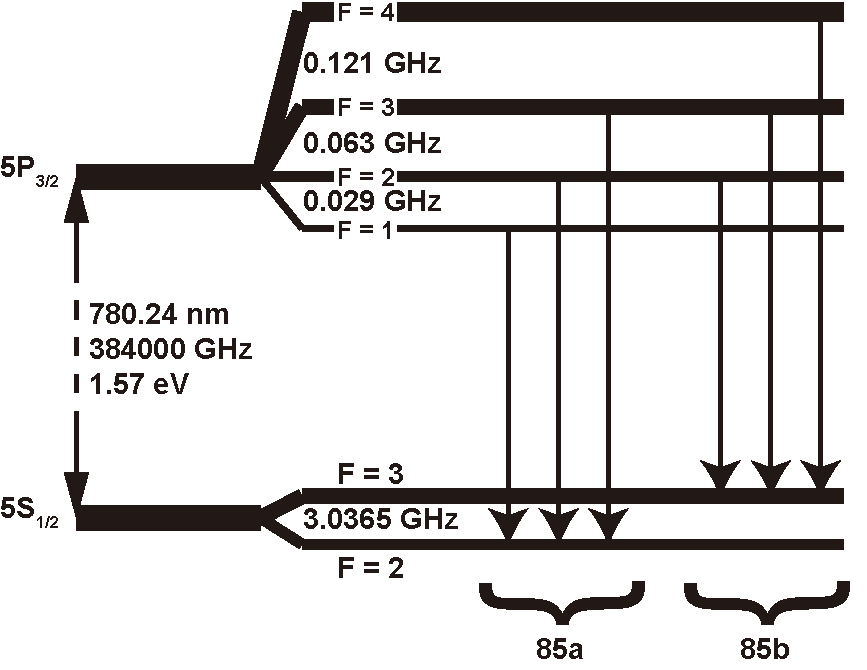
\includegraphics[width=0.45\columnwidth]{EnergyState-85.pdf}}
    \subfigure[$^{87}$Rb]{
    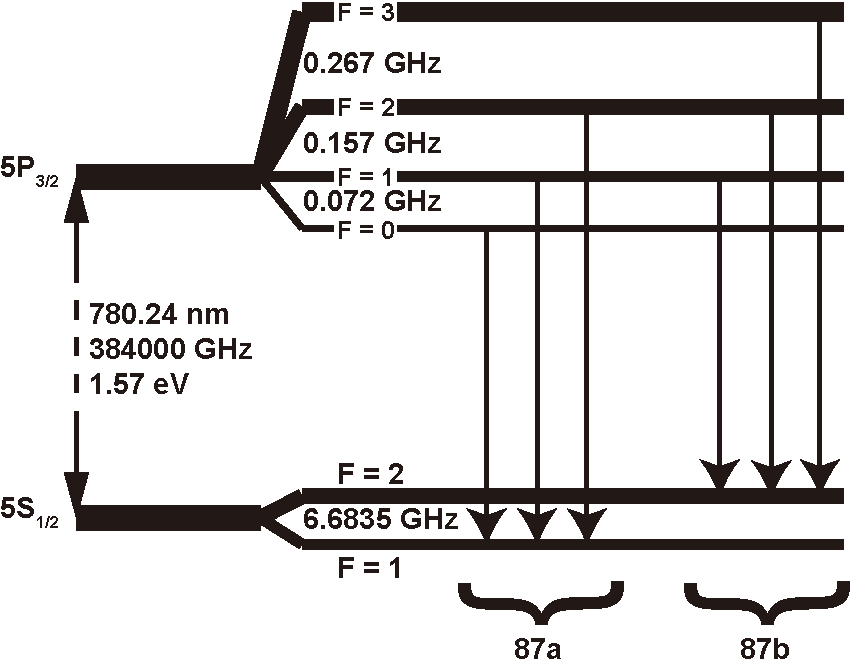
\includegraphics[width=0.45\columnwidth]{EnergyState-87.pdf}}
    \caption{无外界磁场条件下$^{85}$Rb和$^{87}$Rb的部分能级和选择定则允许的跃迁过程.}
    \label{energy-state}
\end{figure}

根据跃迁的选择定则,
\begin{align}
    \Delta F=0,\pm 1,
\end{align}
从$5P_{3/2}$态到$5P_{1/2}$态存在如图\ref{energy-state}所示的跃迁,其中$^{85}$Rb的终态$F=2$的跃迁对应的一系列谱线标号为$85$a,终态$F=3$的跃迁对应的一系列谱线标号为$^{85}$b,$^{87}$Rb的终态$F=1$的跃迁对应的一系列谱线标号为$87$a,终态$F=2$的跃迁对应的一系列谱线标号为$87$b. 每种标号的谱线系实际上各包含三条谱线,但在无饱和吸收的情况下,同一个谱线系中的三条谱线因增宽而相互重叠(详述于下一小小节),在光谱上只表现为一个峰,如图\ref{theoretical-absorption}所示.

\begin{figure}[H]
    \centering
    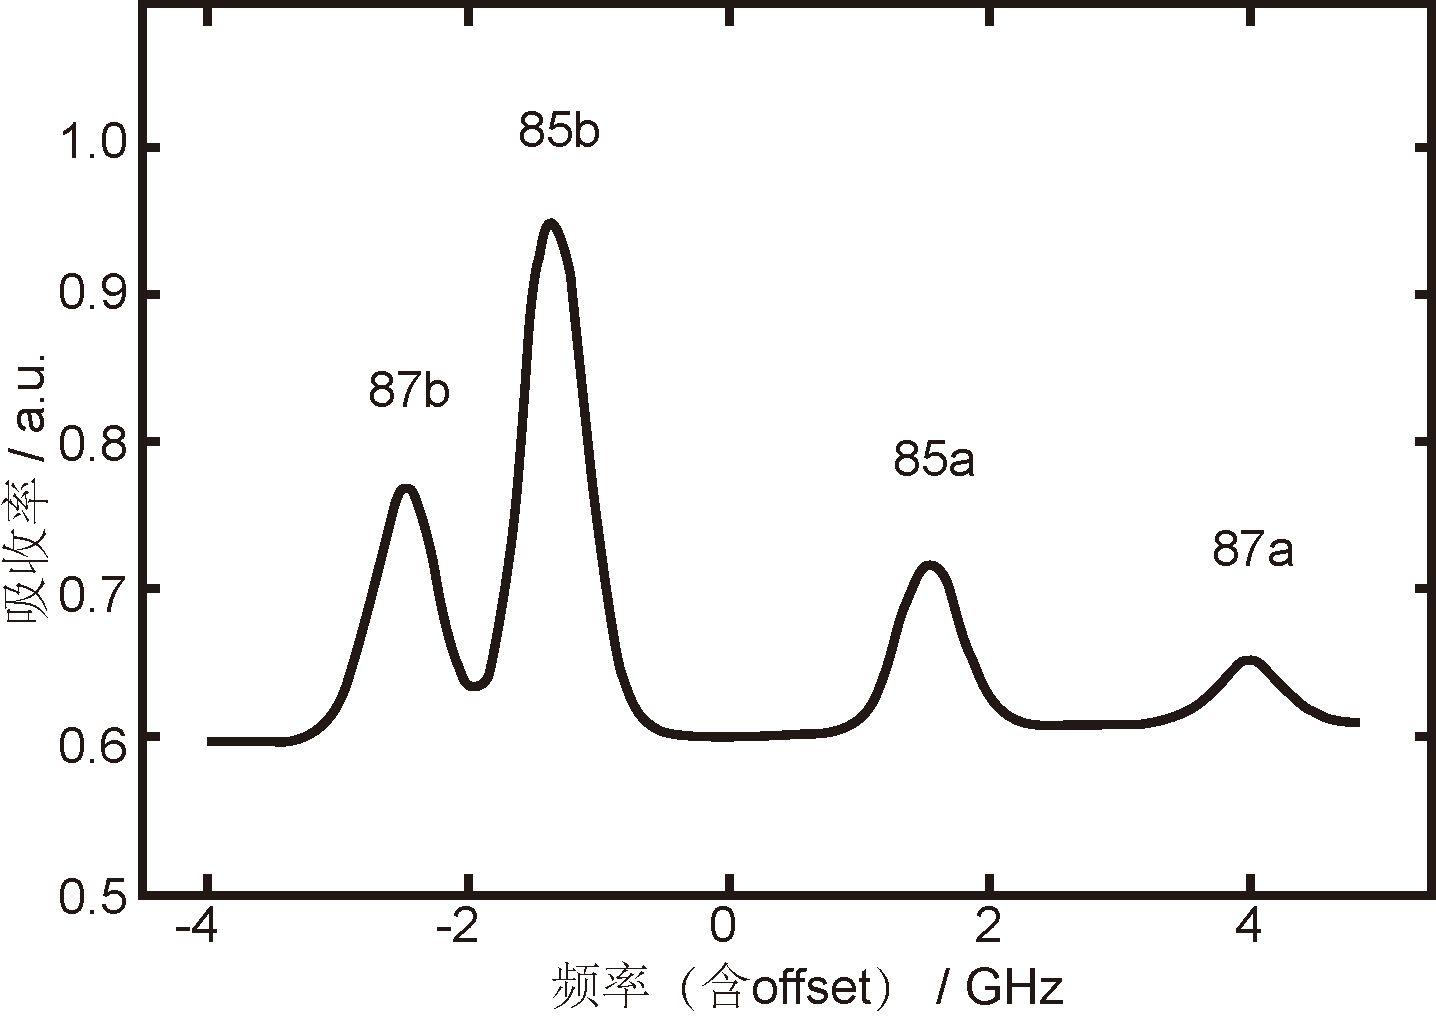
\includegraphics[width=.9\columnwidth]{TheoreticalAbsorption.png}
    \caption{铷蒸汽吸收谱的理论线型.}
    \label{theoretical-absorption}
\end{figure}

\subsubsection{光谱增宽}
实验中测得的铷原子谱线并非分立的狄拉克函数状的特征峰,而是存在由不确定性原理和有限的能级寿命共同导致的洛伦兹增宽和由热运动的原子的多普勒效应导致的多普勒增宽. 下面我们分别来讨论这两种增宽.

\subsubsubsection{自然增宽}
自然增宽来源于有限的能级寿命. 根据不确定性原理,能级的增宽与其平均寿命存在如下关系:
\begin{align}
    \Delta E\cdot\Delta t\geq\frac{\hbar}{2\pi}.
\end{align}
即有限的能级寿命必然导致能级的增宽,从而反映在测得的谱线上.

利用一个半经典的模型,我们可以推导出这一增宽的线型. 设想仅存在一高一低两个能级,在单位时间内,原子自发辐射而从高能级跃迁至低能级的概率是常数,因此高能级上的原子数量随着时间指数衰减,而单位时间内自发辐射的原子数亦随时间指数衰减,从而辐射的电磁波强度亦随时间指数衰减,其电/磁场分量可表为
\begin{align}
    u(t)=u_0e^{-\frac{t}{2T}}e^{i2\pi\nu_0t},
\end{align}
其中$u_0$为初始场强,$T$为高能级的寿命,也是光强衰减为其初始值的$1/e$所需的时间,$\nu_0$为两能级之间的共振频率.
利用傅里叶变换,辐射的电磁场可展开为各频率简谐波的叠加
\begin{align}
    u(t)=\int_{-\infty}^{+\infty}U(\nu)e^{i2\pi\nu t}\,d\nu,
\end{align}
其中角频率为$\omega$的电磁场分量为
\begin{align}
    U(\nu)=\int_{-\infty}^{+\infty}u(t)e^{-i2\pi\nu t}\,d\tau.
\end{align}
考虑到当$t<0$时,自发辐射尚未开始,$u(t)=0$,上式可化为
\begin{align}
    u(\nu)=\int_0^{+\infty}u_0e^{-\frac{t}{2T}}e^{-i2\pi(\nu-\nu_0)t}\,d\tau=\frac{u_0}{i2\pi(\nu-\nu_0)+1/2T}.
\end{align}
光强正比于电磁场的平方,故频率为$\nu$的分量的光强具有如下的形式:
\begin{align}
    I(\nu)\propto\abs{u(\nu)}^2\propto\frac{1}{4\pi^2(\nu-\nu_0)^2+1/(2T)^2}.
\end{align}
归一化后可得相对光强(单位频率范围内光强在总光强中的占比):
\begin{align}
    f_N(\nu)=\frac{1/T}{4\pi^2(\nu-\nu_0)^2+(1/2T)^2}=\frac{\Delta\nu_N/2\pi}{(\nu-\nu_0)^2+(\Delta\nu_N/2)^2},
\end{align}
其中半高宽
\begin{align}
    \label{nature-width}
    \Delta\nu_N=\frac{1}{2\pi\tau}.
\end{align}
此即自然增宽的线型函数,为一洛伦兹型函数.

一般原子激发态的平均寿命数量级在$10^{-5}-10^{-8}$ s范围内,故自然增宽的数量级大致在$10^{-4}\sim 10^{-1}$ GHz范围内.

\subsubsubsection{多普勒增宽}
多普勒增宽来自于气体中热运动的原子的多普勒效应. 对于较为稀薄的气体,我们可以将其视为遵循玻尔兹曼统计的理想气体,由此可以得到其多普勒增宽的线型.

设气体含有$N$个原子,体积为$V$. 每个原子的平动动能为
\begin{align}
    \epsilon=\frac{1}{2m}(p_x^2+p_y^2+p_z^2).
\end{align}
其中$m$为单个气体原子的质量,$p_x,p_y,p_z$分别为气体原子在三个正交方向上的动量大小.
假设平均每个平动状态所占据相空间中的体积为$h_0^3$,则在体积$V$,动量范围$dp_xdp_ydp_z$对应的相空间中,所能容纳的平动状态数为$\frac{V}{h_0^3}dp_x\,dp_y\,dp_z$.
因此能量为$\epsilon$的原子数为
\begin{align}
    dN=A\frac{V}{h_0^3}e^{-\epsilon/k_BT}dp_x\,dp_y\,dp_z
\end{align}
其中$k_B$为玻尔兹曼常数,$T$为气体的温度,$A$为一常数.
由总原子数
\begin{align}
    N=\int_{-\infty}^{+\infty}\int_{-\infty}^{+\infty}\int_{-\infty}^{+\infty}dN=\frac{V}{h_0^3}\frac{1}{8}\left(\frac{2m\pi}{\beta}\right)^{3/2}
\end{align}
得到
\begin{align}
    A=\frac{N}{V}\left(\frac{h_0^2}{2\pi mkT}\right)^{3/2}.
\end{align}
故质心动量在$dp_x\,dp_y\,dp_z$范围内的原子数为
\begin{align}
    dN=N\left(\frac{1}{2\pi mk_BT}\right)^{3/2}e^{-\frac{1}{2k_BmT}\left(p_x^2+p_y^2+p_z^2\right)}\,dp_x\,dp_y\,dp_z.
\end{align}
用速度作为变量代换动量,即$p_x=mv_x$,$p_y=mv_y$,$p_z=mv_z$,有
\begin{align}
    dN=N\left(\frac{m}{2\pi k_BT}\right)^{3/2}e^{-\frac{m}{2k_BT}\left(v_x^2+v_y^2+v_z^2\right)}\,dv_x\,dv_y\,dv_z.
\end{align}
此即麦克斯韦速度分布律,它描述了单位体积内,速度在$dv_x\,dv_y\,dv_z$范围内的原子数:
\begin{align}
    dn=\frac{N}{V}\left(\frac{m}{2\pi k_BT}\right)^{3/2}e^{-\frac{m}{2k_BT}\left(v_x^2+v_y^2+v_z^2\right)}\,dv_x\,dv_y\,dv_z.
\end{align}
由于在相同速度下,纵向多普勒效应远比横向多普勒效应显著,因此我们只需考虑一维(激光传播方向,设为$z$轴方向)上的多普勒效应. $z$轴方向速度分量在$v_z\sim v_z+dv_z$范围内的原子数在总原子数中的占比为
\begin{align}
    \frac{V\,dn_z}{N}=\left(\frac{m}{2\pi k_BT}\right)^{1/2}e^{-\frac{mv_z^2}{2k_BT}}\,dv_z,
\end{align}
根据多普勒效应,这部分原子所吸收和辐射的光子频率为
\begin{align}
    \nu=\frac{1-v/c}{\sqrt{1-v^2/c^2}}\nu_0,
\end{align}
其中$\nu_0$为静止原子的能级跃迁频率. 由于气体原子运动速度远小于光速$c$,故有近似:
\begin{align}
    \nu=\left(1-\frac{v}{c}\right)\nu_0.
\end{align}
这部分原子吸收或辐射的光强在总光强中的占比即为对应的原子数占比
\begin{align}
    \notag f_D(\nu)\,d\nu=&\frac{V\,dn_z}{N}\\
    =&\left(\frac{m}{2\pi k_BT}\right)^{1/2}\exp\left[-\frac{mc^2(\nu-\nu_0)^2}{2k_BT\nu_0^2}\right]\frac{c}{\nu_0}\,d\nu,
\end{align}
故相对光强为
\begin{align}
    \nonumber f_D(\nu)=&\left(\frac{m}{2\pi k_BT}\right)^{1/2}\exp\left[-\frac{mc^2(\nu-\nu_0)^2}{2k_BT\nu_0^2}\right]\frac{c}{\nu_0}\\
    =&\frac{2}{\Delta\nu_D}\left(\frac{\ln 2}{\pi}\right)^{1/2}\exp\left\{-\left[4\ln 2\left(\frac{\nu-\nu_0}{\Delta\nu_D}\right)^2\right]\right\},
\end{align}
其中半高宽
\begin{align}
    \label{Doppler-width}
    \Delta\nu_D=2\nu_0\left(\frac{2k_BT}{mc^2}\ln 2\right)^{1/2}.
\end{align}
此即多普勒增宽的光谱线型函数,为一高斯型函数. 将式\eqref{Doppler-width}中各常数代入可得
\begin{align}
    \Delta\nu_D=7.16\times 10^{-7}\sqrt{T/\mu_{\text{mol}}}\nu_0,
\end{align}
其中$\mu_{\text{mol}}$为原子量. 以铷原子为例,$\mu_{\text{mol}}=85.5$,$^2$P$_{3/2}$态和$^2$S$_{1/2}$态间跃迁频率为$384000$ GHz,在常温($300$ K)下,其多普勒增宽约为$0.5$ GHz,远大于自然增宽,故光谱的增宽以多普勒增宽为主导.

\subsubsubsection{综合增宽}

实际的光谱增宽同时来自上述两种增宽机制的综合贡献,如图\ref{broadening}所示:热运动的原子的速度满足麦克斯韦速度分布率(高斯分布),而处于各个速度的原子各自辐射出指数衰减的电磁波,因此处于各个速度的原子都对总光谱贡献洛伦兹线型的子光谱(图中红线),这些子光谱按照高斯型的权重(图中绿线)叠加成总光谱(图中蓝线),总光谱线型函数为自然增宽线型函数和多普勒增宽线型函数的卷积:
\begin{align}
    f(\nu)=\int_{-\infty}^{+\infty}f_L(\nu')f_D(\nu-\nu')\,d\nu'.
\end{align}
这一线型称为Voigt线型.

\begin{figure}[H]
    \centering
    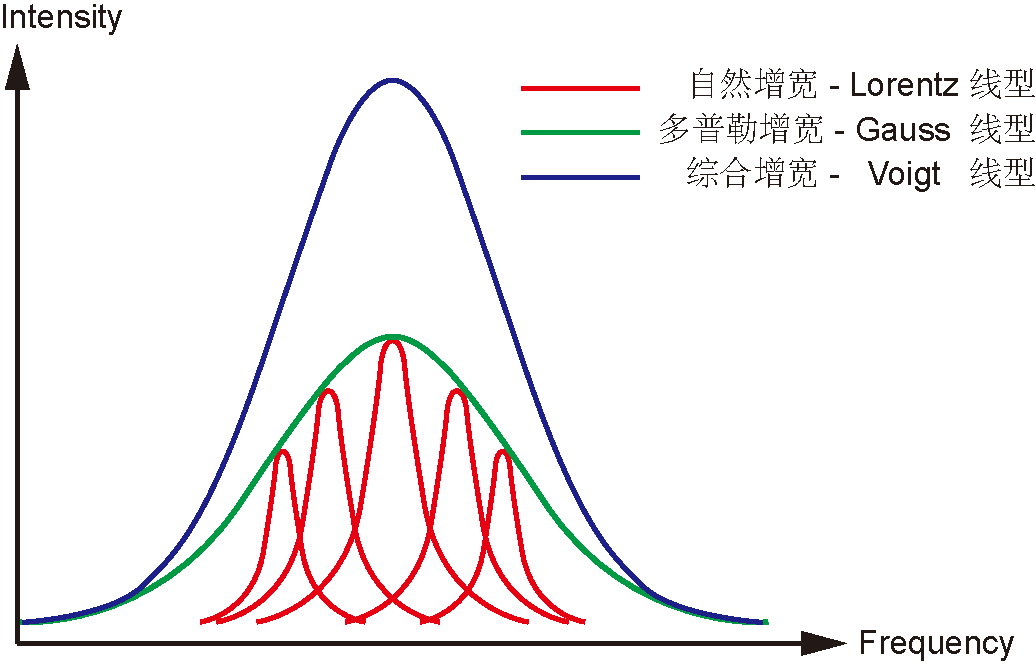
\includegraphics[width=.9\columnwidth]{Broadening.png}
    \caption{综合增宽机制示意图:各洛伦兹线型子光谱以高斯线型权重叠加成Voigt线型总光谱.}
    \label{broadening}
\end{figure}

由于常温下气体光谱增宽的量级($\sim 10^{-1}$ GHz)大于铷原子5P$_{3/2}$能级的超精细结构劈裂($10^{-2}\sim 10^{-1}$ GHz),故根据瑞利判据,即使是用单色性极好的激光,我们也无法在单纯的吸收谱上分辨出P轨道劈裂对应的超精细结构.

\subsection{饱和吸收法}
为了在常温下测得铷原子的超精细结构,我们需要消除多普勒增宽的影响,一个有效的方法是采用饱和吸收光谱技术. 饱和吸收光谱是将同频率的、增宽远小于气体多普勒增宽的一束泵浦光和和一束探测光从同一条路径、两个相反的方向入射气体,通过扫描两束激光的频率而测得的探测光光谱.

\subsubsection{饱和吸收法的基本原理}
由于多普勒效应,沿着光路具有速度分量的原子感受到的泵浦光和探测光具有不同的频率,而沿着光路速度分量为零的原子感受到到的泵浦光和探测光具有相同的频率. 如图\ref{saturated-absorption}所示,假设泵浦光从左入射气体,而探测光从右入射气体,两束激光光路重合. 若仅考虑原子在能量差为$h\nu$的两个能级之间的跃迁,当泵浦光和探测光的频率与原子的共振频率失谐,为$(\nu-\delta\nu)$,则从左入射气体的泵浦光仅激发以$\frac{\delta\nu}{\nu_0}c$向左运动的原子,吸收从右传入射气体的探测光的则是以$\frac{\delta\nu}{\nu_0}c$向左运动的原子,因此泵浦光不影响探测光的吸收强度,光谱强度与无饱和吸收的光谱相等;若泵浦光和探测光与原子在两个能级间的跃迁共振,即其频率为$\nu_0$,则两束光均与静止的原子发生相互作用,由于较强的泵浦光激发将近半数的原子激发至激发态,能吸收探测光的基态原子数量就相应减少,因此吸收强度较无饱和吸收的更小,饱和吸收光谱在$\nu_0$处产生了一个“烧孔”. 由于在烧孔处的吸收强度的减弱仅由静止的这一部分原子所贡献,因此这些烧孔的半“深”宽应与自然增宽的半高宽相同.

\begin{figure}[H]
    \centering
    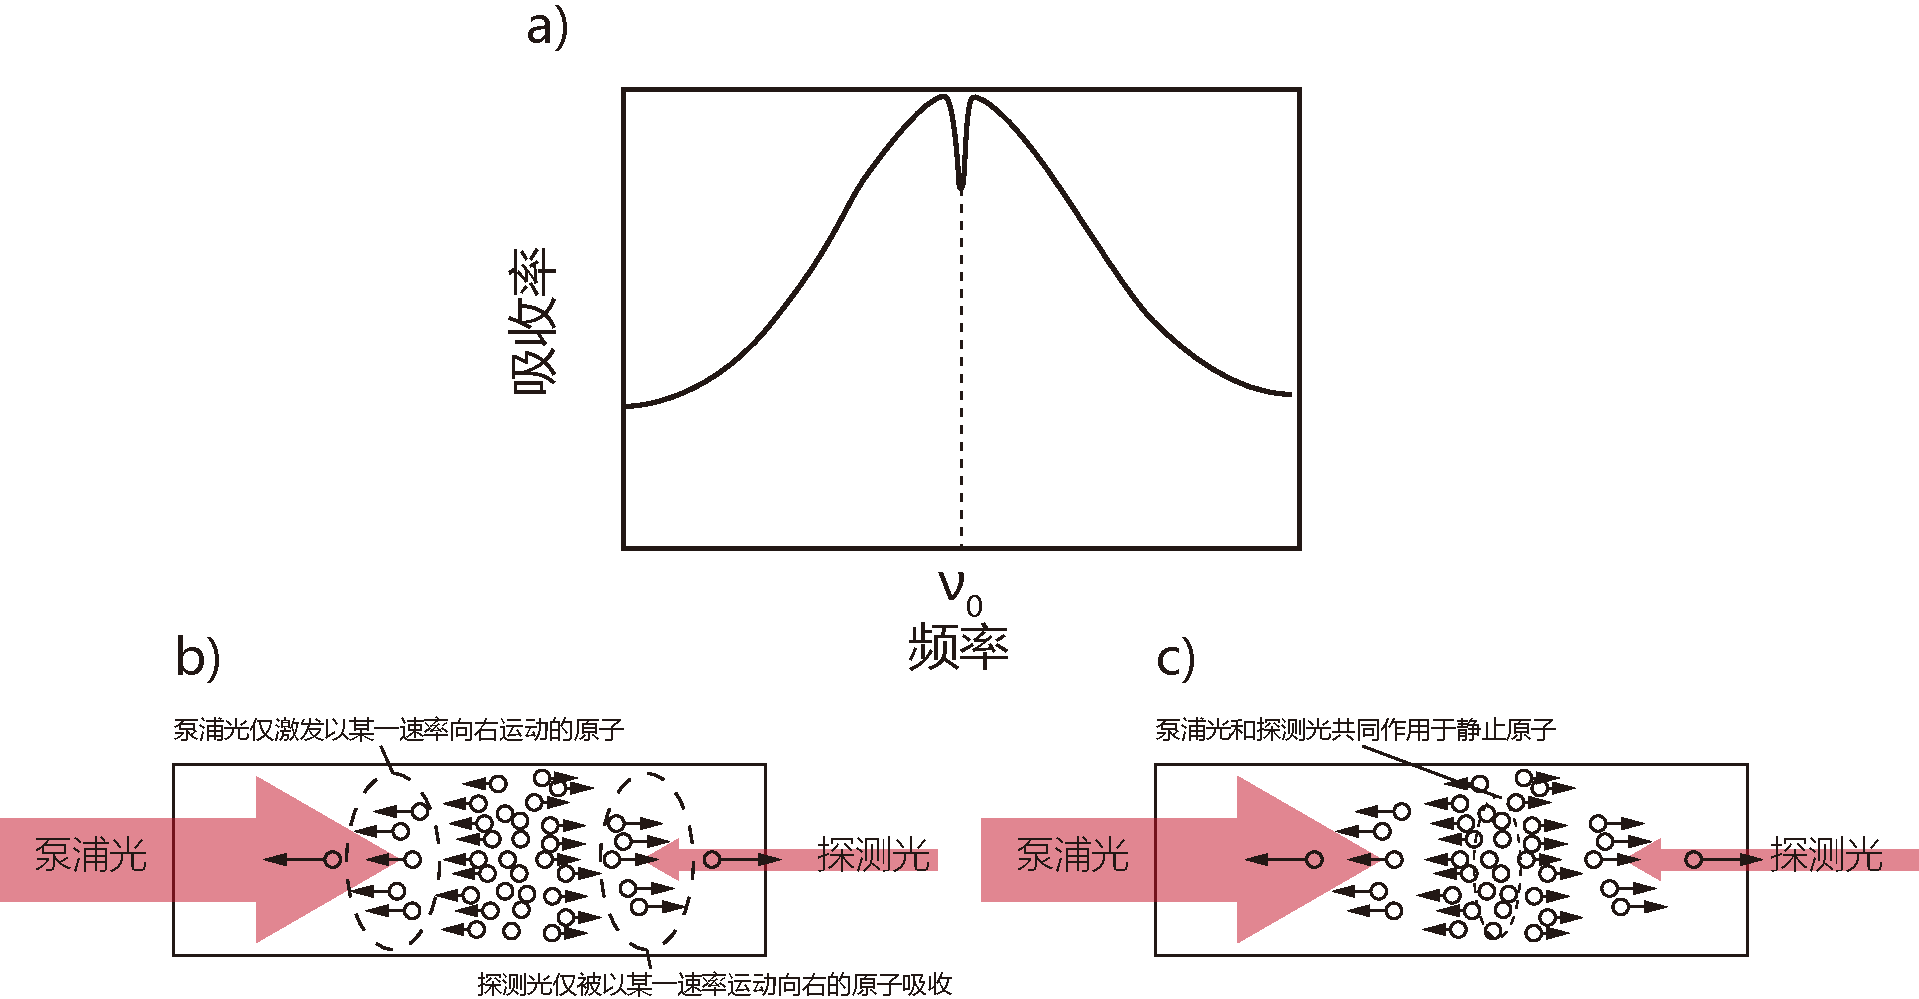
\includegraphics[width=.95\columnwidth]{SaturatedAbsorption.png}
    \caption{饱和吸收光谱原理示意图. (a) 饱和吸收光谱理论线型,(b) 当入射激光频率略小于跃迁频率,激光与气体中原子的作用机制示意图,(c) 当入射光频率等于跃迁频率时,激光与气体中原子的作用机制示意图.}
    \label{saturated-absorption}
\end{figure}

\subsubsection{交叉共振现象}
实验中测得饱和吸收光谱除了在原子能级跃迁的共振频率处存在烧孔,还可能在某两个跃迁频率$\nu_1$和$\nu_2$的中点$(\nu_1+\nu_2)/2$处也存在烧孔,这一现象称为交叉共振(crossover resonance).

交叉共振现象是由原子不同能级跃迁的耦合造成的. 如图\ref{crossover-resonant}(a)所示,以一个V型的三能级系统为例,原子可以由基态$0$吸收$h\nu_1$的能量向激发态$1$跃迁,或吸收$h\nu_2$的能量向激发态$2$跃迁,而由于选择定则的限制,原子不能在两个激发态之间跃迁. 如图\ref{crossover-resonant}(b)所示,当入射的泵浦光和探测光的频率为$(\nu_1+\nu_2)/2$时,对于以速率$(\nu_2-\nu_1)c/2(\nu_1+\nu_2)$向左运动的原子,其感受到泵浦光的频率为$\nu_2$而感受到探测光的频率为$\nu_1$,故这部分原子大部分被泵浦光激发至激发态$2$,而对探测光的吸收较无泵浦光时更弱,而对于以速率$(\nu_2-\nu_1)c/2(\nu_1+\nu_2)$向右运动的原子,其感受到泵浦光的频率为$\nu_1$而感受到探测光的频率为$\nu_2$,故这部分原子大部分被泵浦光激发至激发态$1$,而对探测光的吸收较无泵浦光时更弱,因此饱和吸收光谱在$(\nu_1+\nu_2)/2$处产生一个额外的烧孔,如图\ref{crossover-resonant}(c)所示.

交叉共振并非总是导致吸收谱在中点频率处吸收强度的降低. 对于$\Lambda$型的三能级系统,我们可以同理预测,吸收谱在中点频率处存在一个凸起,而非一个烧孔,如图\ref{crossover-resonant}(d)所示.

因为交叉共振的烧孔由两批不同速度的原子贡献,因此其烧孔大小往往较原子原有跃迁频率处的烧孔要大.

\begin{figure}[H]
    \centering
    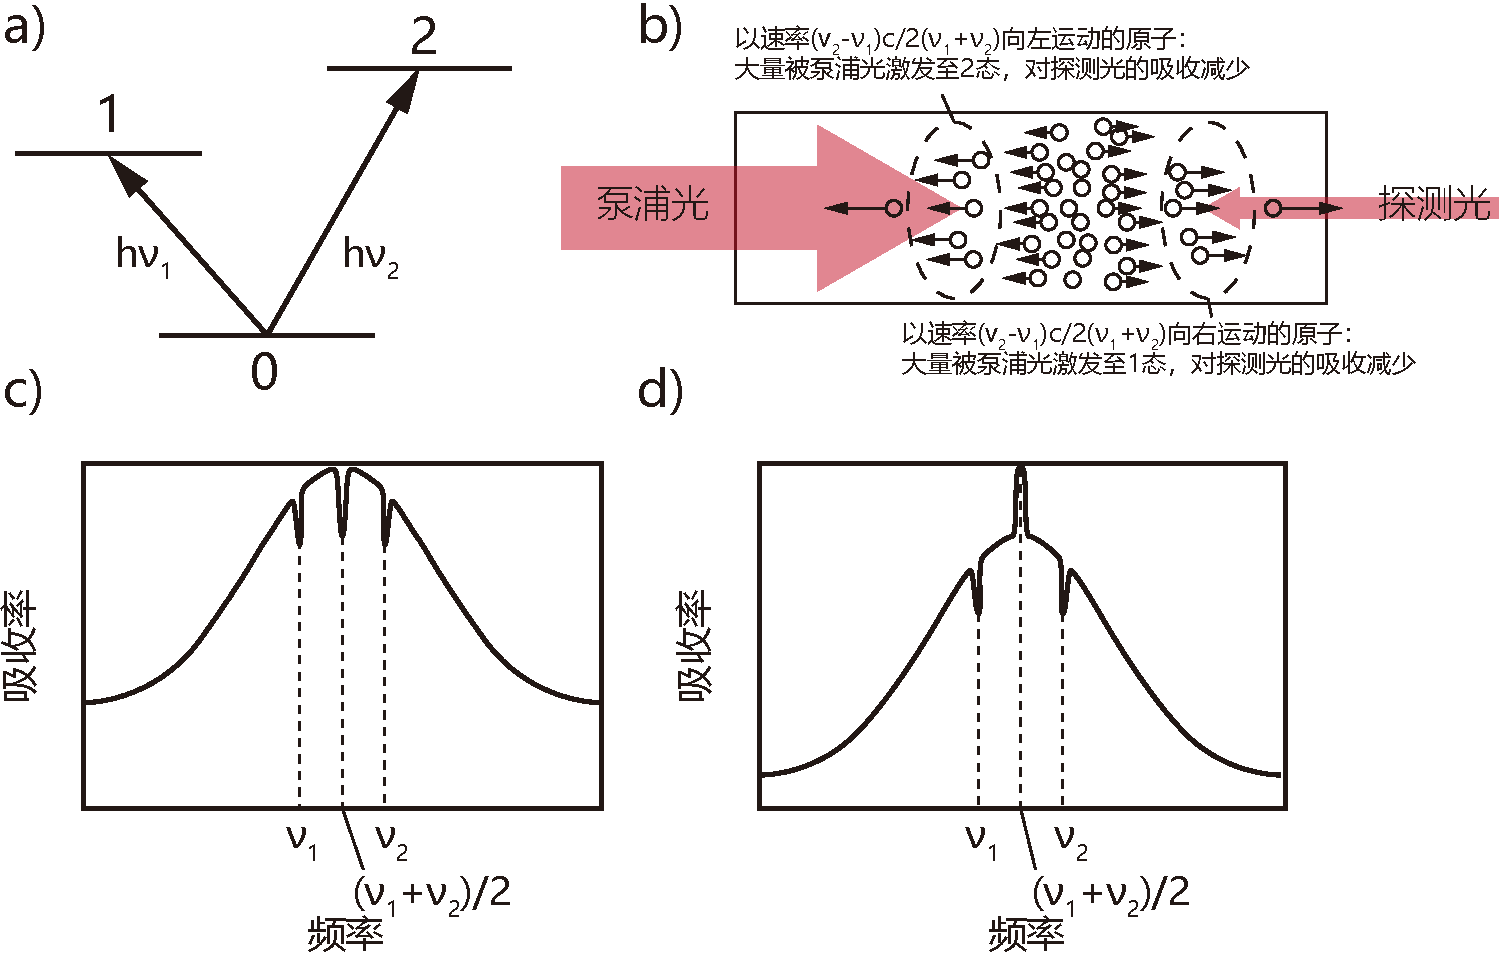
\includegraphics[width=.95\columnwidth]{CrossoverResonant.png}
    \caption{交叉共振现象示意图. (a) V型三能级系统,(b) 当入射激光频率为$(\nu_1+\nu_2)/2$时,激光与气体中原子的作用机制示意图,(c) V型三能级系统的饱和吸收光谱理论线型,(d) $\Lambda$型三能级系统的饱和吸收光谱理论线型.}
    \label{crossover-resonant}
\end{figure}

\subsection{Kramers-Kronig关系及其在气体折射率中的体现}
在入射光较弱的条件下,气体可视为一线性系统,受因果律影响,其响应函数——电极化率的实部和虚部遵循线性系统的一般规律——Kramers-Kronig关系.

\subsubsection{Kramers-Kronig关系}
对于一个具有线性响应$h(t)$的系统,输入信号$x(t)$,则输出信号为响应函数与输入信号的卷积
\begin{align}
    y(t)=h(t)=\int_{-\infty}^{+\infty}h(\tau)x(t-\tau)\,d\tau.
\end{align}
其中响应函数$h(\tau)$的物理意义是,在任意时刻$t$的输入信号$x(t)$总会对$t+\tau$时刻的输出信号产生$h(\tau)x(t+\tau)$的贡献.
根据卷积定理,输出信号的频谱为输入信号频谱和响应函数频谱的乘积
\begin{align}
    Y(\omega)=\mathscr{F}[y(t)]=\mathscr{F}[h(t)]\mathscr{F}[x(t)]=H(\omega)X(\omega).
\end{align}

因果律要求,任意时刻的输入不能影响到之前的输出,因此响应函数在信号输入之前($t<0$处)均为零
\begin{align}
    h(t)=0,\qquad\forall t<0,
\end{align}
从而必可表为如下形式
\begin{align}
    h(t)=\sgn(t)h_o(t)+h_o(t),
\end{align}
其中
\begin{align}
    f_o(t)=\left\{\begin{array}{ll}
        \frac{1}{2}f(t),&t>0,\\
        -\frac{1}{2}f(-t),&t<0,
    \end{array}\right.
\end{align}
为一奇函数,而由于符号函数$\sgn(t)$亦为一奇函数,故$\sgn(t)h_o(t)$为一偶函数. 经过傅里叶变换,得频域中响应函数
\begin{align}
    \notag H(\omega)=&\mathscr{F}[f(t)]=\frac{1}{\sqrt{2\pi}}\mathscr{F}\left[\sgn(t)\right]*H_o(f)+H_o(f)\\
    =&\frac{1}{\pi}\frac{1}{i\omega}*H_o(\omega)+H_o(\omega),
\end{align}
其中
\begin{align}
    H_o(\omega)=\mathscr{F}[h_o(t)].
\end{align}
由于$h_o(t)$为一奇函数,故$H_o(\omega)$为一纯虚数函数,而$\frac{1}{i\omega}*H_o(\omega)$为一实函数. 因此频域中响应函数的实部为
\begin{align}
    \re[H(\omega)]=\frac{1}{\pi}\frac{1}{i\omega}*H_o(\omega),
\end{align}
虚部为
\begin{align}
    \im[H(\omega)]=-iH_o(\omega).
\end{align}
两者之间的关系为
\begin{align}
    \boxed{\re[H(\omega)]=\frac{1}{\pi}\frac{1}{\omega}*\im[H(\omega)].}
\end{align}
此即\textbf{Kramers-Kronig关系}.

\subsubsection{气体折射率中的Kramers-Kronig关系}
我们可以从经典力学和量子力学两个角度分别推导出气体折射率的实部和虚部,并证明两者满足Kramers-Kronig关系.

\subsubsubsection{经典力学图像}
在经典力学的图像中,我们将气体原子中的电子等效为由核束缚的谐振子,从而可以推导出其在交变电场中的电极化强度响应,得到含有大量这种原子的气体的折射率的实部与虚部之间的关系.

无外场作用的情况下,原子中电子绕原子核运动,其平均位置$\bm{x}$与原子核位置(设为原点)重合,即$\bm{x}=0$;在弱场下,可近似认为电子平均位置的偏离正比场强,故可将电子等效为受原子核束缚的一个谐振子,其位移为电子平均位置相对于原子核的偏离$\bm{x}$,其本征振动频率$\omega_0$为电子在能级间跃迁的频率,其阻尼系数设为$2\gamma$(在经典图像中无法得到阻尼系数的具体数值,只能通过实验得到经验值,这里乘$2$没有任何物理意义,单纯为了后面数学上形式更简单). 在一维情况下,该谐振子在电场$E(x,t)$中的动力学方程为
\begin{align}
    \label{motion-equ}
    m\ddot{x}=-eE(x,t)-\omega_0^2x-2\gamma\dot{x},
\end{align}
其中上式右边三项分别为该谐振子受到的驱动力(电场力)、回复力和阻尼力.

对于透过气体传播的电磁波,其在空间中给定某点的电场可表为
\begin{align}
    E(t)=E_0e^{i\omega t}.
\end{align}
从而可解得
\begin{align}
    x(t)=x_0e^{-i\omega t}=-\frac{eE(t)}{m}\frac{1}{(\omega_0^2-\omega^2)-2i\gamma\omega}.
\end{align}

每个原子贡献的偶极矩为
\begin{align}
    p(t)=-ex(t)=\frac{e^2E(t)}{m}\frac{1}{(\omega_0^2-\omega^2)-2i\gamma\omega}.
\end{align}
则气体的电极化矢量为
\begin{align}
    P(t)=\frac{N}{V}p(t)=\frac{e^2NE(t)}{mV}\frac{1}{(\omega_0^2-\omega^2)-2i\gamma\omega}=\epsilon_0\chi E(t).
\end{align}
故电极化率为
\begin{align}
    \chi=\frac{P}{\epsilon_0E}=\frac{e^2N}{\epsilon_0mV}\frac{1}{(\omega_0^2-\omega^2)-2i\gamma\omega}.
\end{align}
事实上,若仔细思考,上面得到的电极化率的表达式并非是完全准确的,例如,原子中往往存在不止一个电子,电子的有效电荷、有效质量也不一定是$e$、$m$(所幸的是,表达式的形式是没有错的,只是系数上存在一定偏差,我们将在下一小小小节尝试用量子力学的方法严谨地推导电极化率),故为了修正电极化率的表达式,我们引入一个经验系数$f$(又称振子强度),从而将电极化率表为
\begin{align}
    \chi=\frac{4\pi Nfe^2}{mV}\frac{1}{(\omega_0^2-\omega^2)-2i\omega\gamma}
\end{align}

作为非磁性介质,气体的折射率为
\begin{align}
    n=\sqrt{\epsilon_r}=\sqrt{1+\chi}.
\end{align}
对于较小的电极化率,上式可近似为
\begin{align}
    \notag n\approx 1+\frac{\chi}{2}=&1+\frac{2\pi Nfe^2}{mV}\frac{1}{(\omega_0^2-\omega^2)-i\omega\gamma}\\
    =&1+\frac{2\pi Nfe^2}{mV}\frac{(\omega_0^2-\omega^2)+2i\omega\gamma}{(\omega_0^2-\omega^2)^2+4\omega^2\gamma^2}.
\end{align}
将折射率写成实部与虚部相加的形式
\begin{align}
    n=n_0(1+i\kappa),
\end{align}
则有
\begin{align}
    n_0=1-\frac{2\pi Nfe^2}{mV}\frac{\omega^2-\omega_0^2}{(\omega^2-\omega_0^2)^2+4\omega^2\gamma^2},
\end{align}
及
\begin{align}
    n_0\kappa=\frac{2\pi Nfe^2}{mV}\frac{\omega\gamma}{(\omega^2-\omega_0^2)^2+4\omega^2\gamma^2}.
\end{align}
当电磁场振荡频率与谐振子的本征频率相近(如本实验中入射激光的频率在铷原子共振频率附近扫描),$\omega\approx\omega_0$,上面两式还可进一步近似为
\begin{align}
    \notag n_0=&1-\frac{2\pi Nfe^2}{mV}\frac{\frac{(\omega+\omega_0)(\omega-\omega_0)}{\omega_0(\omega+\omega_0)}}{\frac{(\omega+\omega_0)^2(\omega-\omega_0)^2+4\omega^2\gamma^2}{\omega_0(\omega+\omega_0)}}\\
    \notag\approx&1-\frac{2\pi Nfe^2}{mV}\frac{(\omega-\omega_0)/\omega_0}{2(\omega-\omega_0)^2+2\gamma^2}\\
    =&1-\frac{\pi Nfe^2}{mV}\frac{\Delta\omega/\omega_0}{\Delta\omega^2+\gamma^2},
\end{align}
和
\begin{align}
    \notag n_0\kappa=&\frac{2\pi Nfe^2}{mV}\frac{\frac{2\omega\gamma}{\omega_0(\omega+\omega_0)}}{\frac{(\omega+\omega_0)^2(\omega-\omega_0)^2+4\omega^2\gamma^2}{\omega_0(\omega+\omega_0)}}\\
    \notag\approx&\frac{2\pi Nfe^2}{mV}\frac{\gamma/\omega_0}{2(\omega-\omega_0)^2+2\gamma^2}\\
    =&\frac{\pi Nfe^2}{mV}\frac{\gamma/\omega_0}{\Delta\omega^2+\gamma^4}.
\end{align}

理论上说,电磁波的磁场也应对振子产生作用(洛伦兹力),而在上面的推导中,我们却忽略了这一项,这是因为电子在电磁波中受到洛伦兹力的量级远小于电场力的量级. 我们可以通过简单的估算说明这一点. 假设电磁波中的电场强度最大值为$1$V/m,则电子受到电场力大小为
\begin{align}
    F_{\text{electric}}=eE=1.6\times 10^{-19}\text{C}\times 1\text{V/m}=1.6\times 10^{-19}\text{N}.
\end{align}
磁感应强度$\bm{B}$与电场$\bm{E}$具有如下关系
\begin{align}
    \bm{B}=\frac{\bm{k}}{\omega}\times\bm{E}.
\end{align}
其中$\bm{k}$为电磁波的波矢,$\omega$为电磁波的角频率.
在真空中,
\begin{align}
    B=\frac{E}{c}=\frac{1\text{V/m}}{3\times 10^8\text{m/s}}=\frac{1}{3}\times 10^{-8}\text{T}.
\end{align}
我们用玻尔模型估算原子中电子的运动速度. 玻尔模型中,氢原子的电子和原子核之间的库仑力提供向心力使电子绕原子核旋转:
\begin{align}
    \label{Bohr-1}
    m\frac{v^2}{r}=\frac{1}{4\pi\epsilon_0}\frac{e^2}{r^2}.
\end{align}
其中$v$为电子的线速率,$r$为电子轨道半径,$\epsilon_0$为真空中介电常数. 根据玻尔的假设,电子轨道的周长是其波长的整数倍
\begin{align}
    2\pi r=n\lambda=n\frac{h}{p}=n\frac{h}{mv},
\end{align}
从而
\begin{align}
    r=\frac{\hbar}{mv}.
\end{align}
将上式代入式\eqref{Bohr-1}中解得电子运动速率
\begin{align}
    v=\frac{1}{4\pi\epsilon_0}\frac{e^2}{\hbar}=2.2\times 10^6\text{m/s}.
\end{align}
故电子受到的洛伦兹力最大值为
\begin{align}
    F_{\text{Lorentz}}=evB=1.2\times 10^{-21}\text{N},
\end{align}
比电场力小了两个数量级,故在本小小小节(以及下一小小小节)的模型中我们可以忽略磁场的影响.

\subsubsection{量子力学图像}
在量子力学的图像中,我们利用刘维尔-冯·诺依曼方程(liouville - von neumann equation)求解二能级系统在交变电场中的电极化强度响应,得到气体折射率实部与虚部关系.

假设原子为一个二能级系统,其要么处于能量为$E_1$的基态$\lvert 1\rangle$,要么处于能量为$E_2$的激发态$\lvert 2\rangle$. 在$t=0$时刻及之前,无外场的情况下,气体中的原子满足玻尔兹曼分布,其密度矩阵可表为
\tiny
\begin{align}
    \label{density-matrix-init-value}
    \notag\hat{\rho}(t)=&\frac{1}{1+\exp[-(E_2-E_1)/k_BT]}\lvert 1\rangle\langle 1\rvert+\frac{\exp[-(E_2-E_1)/k_BT]}{1+\exp[-(E_2-E_1)/k_BT]}\lvert 2\rangle\langle 2\rvert,\\
    =&\frac{1}{1+\exp(-\hbar\omega_{21}/k_BT)}\lvert 1\rangle\langle 1\rvert+\frac{\exp(-\hbar\omega_{21}/k_BT)}{1+\exp(-\hbar\omega_{21}/k_BT)}\lvert 2\rangle\langle 2\rvert,\qquad t\leq 0.
\end{align}
\normalsize
其中原子的共振频率
\begin{align}
    \omega_{21}=\frac{E_2-E_1}{\hbar}.
\end{align}

$t=0$时刻开始入射一电磁波,其电场分量表为
\begin{align}
    \bm{E}(t)=\bm{E}_0e^{i\omega t}.
\end{align}
在弱场条件下,可做偶极近似,微扰哈密顿量仅非对角矩阵元非零:
\begin{align}
    \label{perturbed-Hamiltonian}
    \notag\hat{H}_I(t)=&-\hat{\bm{p}}\cdot\bm{E}(t)=\hat{1}\left[-\hat{\bm{p}}\cdot\bm{E}(t)\right]\hat{1}\\
    \notag=&\sum_{m=1,2}\lvert m\rangle\langle m\rvert\left[\hat{\bm{p}}\cdot\bm{E}(t)\right]\sum_{l=1,2}\lvert l\rangle\langle l\rvert\\
    =&-p_{12}E_0e^{i\omega t}\lvert 1\rangle\langle 2\rvert-p_{21}E_0e^{i\omega t}\lvert 2\rangle\langle 1\rvert.
\end{align}
其中$\hat{\bm{p}}$为电偶极矩算符,其在基底$\{\lvert 1\rangle,\lvert 2\rangle\}$上展开的矩阵元为
\begin{align}
    p_{ml}=\langle m\rvert\hat{p}\rvert l\rangle.
\end{align}

相互作用绘景下的密度矩阵为
\begin{align}
    \hat{\rho}'(t)=\hat{U}_0(-t)\hat{\rho}(t)\hat{U}_0(t),
\end{align}
微扰哈密顿量为
\begin{align}
    \hat{U}_I'(t)=\hat{U}_0(-t)\hat{H}_I(t)\hat{U}_0(t),
\end{align}
其中时间演化算符
\begin{align}
    U_0(t)=\exp\left[-\frac{i}{\hbar}\int_0^t\hat{H}_0\,d\tau\right].
\end{align}
将密度矩阵展开为关于微扰的各阶近似:
\begin{align}
    \hat{\rho}(t)'=\hat{\rho}^{'(0)}(t)+\hat{\rho}^{'(1)}(t)+\hat{\rho}^{'(2)}(t)+\cdots,
\end{align}
代入刘维尔方程中
\begin{align}
    \frac{d}{dt}\hat{\rho}'=-\frac{i}{\hbar}[\hat{H}_I,\hat{\rho}'],
\end{align}
方程两边相同阶数的项取等得
\begin{align}
    \frac{d}{dt}\hat{\rho}^{'(0)}(t)=&0,\\
    \frac{d}{dt}\hat{\rho}^{'(n)}(t)=&-\frac{i}{\hbar}\left[\hat{H}',\hat{\rho}^{'(n-1)}\right],\qquad n\geq 1,
\end{align}
积分得相互作用绘景中密度矩阵的零阶近似项保持其初始值不变
\begin{align}
    \hat{\rho}^{'(0)}(t)=\hat{\rho}^{'(0)}(0)=\hat{U}_0(-0)\hat{\rho}(0)\hat{U}_0(0)=\hat{\rho}^{(0)}(0).
\end{align}
而一阶近似项随着时间的演化为
\begin{align}
    \notag\hat{\rho}^{'(1)}(t)=&\left(-\frac{i}{\hbar}\right)\int_0^td\tau_1\,[\hat{H}_I'(\tau_1),\hat{\rho}^{'(0)}(t)],\\
    =&\left(-\frac{i}{\hbar}\right)\int_0^td\tau_1\,[\hat{H}_I'(\tau_1),\hat{\rho}^{(0)}(0)].
\end{align}
故在薛定谔绘景中,
\tiny
\begin{align}
    \hat{\rho}^{(0)}(t)=&\hat{\rho}^{(0)}(0),\\
    \notag\hat{\rho}^{(0)}(t)=&\hat{U}_0(t)\hat{\rho}^{(0)}(t)\hat{U}_0(-t)\\
    \notag=&\left(-\frac{i}{\hbar}\right)\hat{U}_0(t)\int_0^td\tau_1\,[\hat{H}_I'(\tau_1),\hat{\rho}^{(0)}(0)]\hat{U}_0(-t)\\
    =&\left(-\frac{i}{\hbar}\right)\int_0^t\,d\tau_1\hat{U}_0(t-\tau_1)\left[\hat{H}_I(\tau_1)\hat{\rho}^{(0)}(0)-\hat{\rho}^{(0)}(0)\hat{H}_I(\tau_1)\right]\hat{U}_0(-(t-\tau_1)).
\end{align}
\normalsize
将微扰哈密顿量(式\eqref{perturbed-Hamiltonian})和密度矩阵的初始值(式\eqref{density-matrix-init-value})代入上式,得
\tiny
\begin{align}
    \notag\hat{\rho}^{(1)}(t)=&-\frac{1-\exp(-\hbar\omega_{21}/k_BT)}{1+\exp(-\hbar\omega_{21}/k_BT)}p_{12}E_0\frac{\exp(i\omega t)-\exp[(i\omega_{21}-\Gamma_{21})t]}{\hbar(\omega-\omega_{21}-i\Gamma_{21})}\lvert 1\rangle\langle 2\rvert\\
    &+\frac{1-\exp(-\hbar\omega_{21}/k_BT)}{1+\exp(-\hbar\omega_{21}/k_BT)}p_{21}E_0\frac{\exp(i\omega t)-\exp[-(i\omega_{2}+\Gamma_{21})t]}{\hbar(\omega+\omega_{21}-i\Gamma_{21})}\lvert 2\rangle\langle 1\rvert.
\end{align}
\normalsize
其中
\begin{align}
    \tilde{\Omega}_{21}=&\omega_{21}-i\Gamma_{21}=\frac{E_2-E_1}{\hbar}-i\Gamma_{21},\\
    i\tilde{\Omega}_{12}=&\left(i\tilde{\Omega}_{21}\right)^*,
\end{align}
$\Gamma_{21}>0$为密度矩阵相干矩阵元自发弛豫系数.
当外场作用时间足够长,体系趋于稳定,其密度矩阵的一阶近似项趋于:
\scriptsize
\begin{align}
    \notag\lim_{t\rightarrow+\infty}\hat{\rho}^{(1)}(t)=&-\frac{1-\exp(-\hbar\omega_{21}/k_BT)}{1+\exp(-\hbar\omega_{21}/k_BT)}p_{12}E_0\frac{\exp(i\omega t)}{\hbar(\omega-\omega_{21}-i\Gamma_{21})}\lvert 1\rangle\langle 2\rvert\\
    &+\frac{1-\exp(-\hbar\omega_{21}/k_BT)}{1+\exp(-\hbar\omega_{21}/k_BT)}p_{21}E_0\frac{\exp(i\omega t)}{\hbar(\omega+\omega_{21}-i\Gamma_{21})}\lvert 2\rangle\langle 1\rvert
\end{align}
\normalsize
此时气体的电极化强度大小为(如前所述,考虑的是弱场条件,故仅近似到一阶项)
\tiny
\begin{align}
    \notag\langle\hat{P}\rangle=&\tr\left[\frac{N}{V}\hat{p}\hat{\rho}\right]\approx\tr\left[\frac{N}{V}\hat{p}\left(\hat{\rho}^{(0)}+\hat{\rho}^{(1)}\right)\right]=N\sum_{n=1,2}\langle n\rvert\left[N\hat{p}\left(\hat{\rho}^{(0)}+\hat{\rho}^{(1)}\right)\right]\lvert n\rangle\\
    \notag=&\frac{1-\exp(-\hbar\omega_{21}/k_BT)}{1+\exp(-\hbar\omega_{21}/k_BT)}\frac{V}{N}\abs{p_{12}}^2E_0\exp(i\omega t)\times\\
    &\qquad\qquad\qquad\qquad\qquad\qquad\qquad\qquad\left[\frac{1}{\hbar(\omega+\omega_{21}-i\Gamma_{21})}-\frac{1}{\hbar(\omega-\omega_{21}-i\Gamma_{21})}\right].
\end{align}
\normalsize
当外场的频率接近两个能级之间的跃迁频率,$\omega\approx\omega_{21}$,上式中括号内第一项的绝对值将远小于第二项的绝对值,从而可近似为
\scriptsize
\begin{align}
    \notag\langle\hat{P}\rangle\approx&-\frac{1-\exp(-\hbar\omega_{21}/k_BT)}{1+\exp(-\hbar\omega_{21}/k_BT)}\frac{N}{V}\abs{p_{12}}^2E_0\exp(i\omega t)\frac{1}{\hbar(\omega-\omega_{21}-i\Gamma_{21})}\\
    =&-\frac{1-\exp(-\hbar\omega_{21}/k_BT)}{1+\exp(-\hbar\omega_{21}/k_BT)}\frac{N\abs{p_{12}}^2}{\hbar V}\frac{(\omega-\omega_{21})+i\Gamma_{21}}{(\omega-\omega_{21})^2+\Gamma_{21}^2}E(t).
\end{align}
\normalsize
由此得到气体的电极化率为
\small
\begin{align}
    \chi=\frac{P}{\epsilon_0E}=-\frac{1-\exp(-\hbar\omega_{21}/k_BT)}{1+\exp(-\hbar\omega_{21}/k_BT)}\frac{N\abs{p_{12}}^2}{\hbar V}\frac{(\omega-\omega_{21})+i\Gamma_{21}}{(\omega-\omega_{21})^2+\Gamma_{21}^2}.
\end{align}
\normalsize
对于较小的电极化率,气体的折射率为
\begin{align}
    \notag n=&\sqrt{1+\chi}\approx 1+\frac{\chi}{2}\\
    \notag=&1-\frac{1-\exp(-\hbar\omega_{21}/k_BT)}{1+\exp(-\hbar\omega_{21}/k_BT)}\frac{N\abs{p_{12}}^2}{2\hbar V}\frac{(\omega-\omega_{21})+i\Gamma_{21}}{(\omega-\omega_{21})^2+\Gamma_{21}^2}\\
    =&n_0(1+i\kappa).
\end{align}
其中折射率实部
\begin{align}
    n_0=1-\frac{1-\exp(-\hbar\omega_{21}/k_BT)}{1+\exp(-\hbar\omega_{21}/k_BT)}\frac{N\abs{p_{12}}^2}{2\hbar V}\frac{\omega}{\Delta\omega^2+\Gamma_{21}^2},
\end{align}
折射率虚部(符号或有误,存疑)
\begin{align}
    n_0\kappa=-\frac{1-\exp(-\hbar\omega_{21}/k_BT)}{1+\exp(-\hbar\omega_{21}/k_BT)}\frac{N\abs{p_{12}}^2}{2\hbar V}\frac{\Gamma_{21}}{\Delta\omega^2+\Gamma_{21}^2}
\end{align}
其中$\Delta\omega=\omega-\omega_{21}$.

\subsubsection{气体折射率实部与虚部之间的关系}
弱场下的气体为一线性系统,其输入信号为电场强度$\bm{E})(t)$,输出信号可认为是(或者正比于)其电极化强度$P(t)$,其在频域上的响应函数为电极化率$\chi(\omega)=\frac{E(\omega)}{\epsilon_0P(\omega)}$,其实部为
\begin{align}
    \re[\chi(\omega)]=-C\frac{\omega-\omega_0}{(\omega-\omega_0)^2+\gamma},
\end{align}
虚部为
\begin{align}
    \im[\chi(\omega)]=C\frac{\gamma}{(\omega-\omega_0)^2+\gamma^2},
\end{align}
其中$C$为一常数.
可以验证
\tiny
\begin{align}
    \notag&\frac{1}{\pi}\frac{1}{\omega}*\im[\chi(\omega)]=\frac{1}{\pi}\int_{-\infty}^{+\infty}d\xi\,\frac{1}{\omega-\xi}\cdot C\frac{\gamma}{(\xi-\omega_0)^2+\gamma^2}\\
    \notag=&\lim_{\xi\rightarrow+\infty}\frac{C}{\pi}\frac{1}{2[(\omega-\omega_0)^2+\gamma^2]}\times\\
    \notag&\left\{\gamma\{\ln[(\xi-\omega_0)^2+\gamma^2]-2\ln(\xi-\omega)\}+2\omega\arctan\left(\frac{\xi-\omega_0}{\gamma}\right)\right.\\
    \notag&\qquad\qquad\qquad\qquad\qquad\qquad\qquad\qquad\qquad\qquad\qquad\qquad\qquad\qquad\qquad\qquad+2\omega_0\arctan\left(\frac{\omega_0-\xi}{\gamma}\right)\\
    \notag&-\gamma\ln[(\xi-\omega_0)^2+\gamma^2]+2\ln(\xi-\omega)\}-2\omega\arctan\left(\frac{\xi-\omega_0}{\gamma}\right)\\
    \notag&\qquad\qquad\qquad\qquad\qquad\qquad\qquad\qquad\qquad\qquad\qquad\qquad\qquad\qquad\qquad\qquad\left.-2\omega_0\arctan\left(\frac{\omega_0-\xi}{\gamma}\right)\right\}\\
    =&C\frac{(\omega-\omega_0)}{(\omega-\omega_0)^2+\gamma^2}=\re[\chi(\omega)].
\end{align}
\normalsize
满足Kramers-Kronig关系.

\subsection{Mach-Zehnder干涉仪原理}

气体折射率的实部与虚部分别刻画了气体中的光速减慢和气体对光吸收的效应,因此我们可以使用Mach-Zehnder干涉仪来测量激光通过铷蒸汽的强度和相位变化,从而验证在前一小节中得到的气体折射率实部与虚部之间的关系.

如图\ref{M-Z}为M-Z干涉仪的光路示意图,激光从左边进入干涉仪后,被50-50分束镜1分为A、B两束,分别被反射镜A、B反射,其中B路光束相对A路光束在此过程中还经过了铷蒸汽腔,而后两束激光在50-50分束镜2处再次重合而进入光电二极管,通过光电二极管测量得到干涉光的强度. 铷蒸汽腔对于光束B具有两方面的作用:
\begin{itemize}
    \item 铷蒸汽折射率实部大于空气折射率,因此激光在铷蒸汽中传播相同距离所对应的光程差大于在空气传播所对应的光程差,从而使B路光束获得一附加的相位;
    \item 铷蒸汽具有非零的折射率虚部,其物理意义是对于电磁波的吸收,因此B路光束在经过铷蒸汽腔后其强度将有一定程度的减弱.
\end{itemize}
这两方面的作用均与铷蒸汽的折射率有关,而铷蒸汽的折射率与入射激光的频率有关,因此当我们扫描激光频率时,将得到随着激光频率变化的干涉光强.
\begin{figure}[H]
    \centering
    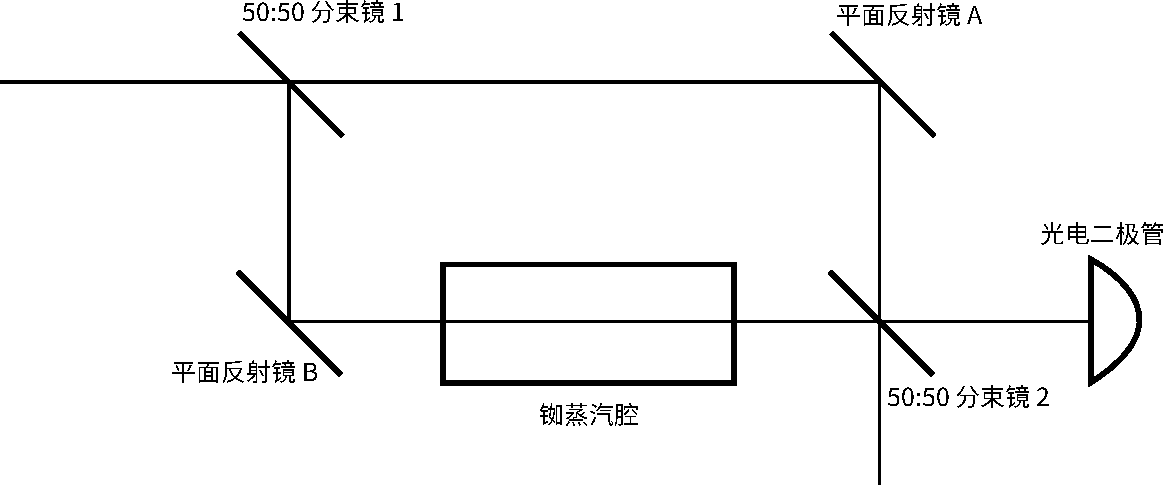
\includegraphics[width=.9\columnwidth]{M-Z-Interferometer.pdf}
    \caption{M-Z干涉仪光路示意图}
    \label{M-Z}
\end{figure}

为了得到干涉光的强度随着激光频率的定量变化关系,我们从无铷蒸汽腔的情况开始讨论. 设激光的频率为$\omega$,入射时电场分量的振幅为$\sqrt{2}E_0$(忽略空气、分光镜和反射镜对激光的衰减和吸收),A、B两路光束走过的距离分别为$L_1$和$L_2$. 假设不存在铷蒸汽腔,则A、B两路光束的电场振幅均为原来的一半,再次叠加时得到的电场分量为
\begin{align}
    E=\frac{E_0}{2}e^{i\frac{\omega}{c}L_1}+\frac{E_0}{2}e^{i\frac{\omega}{c}L_2}.
\end{align}
干涉光强与入射光强的比值为
\begin{align}
    \label{I/I_0-without-cell}
    \frac{I}{I_0}=\frac{\abs{E}^2}{E_0^2}=\frac{1}{2}\left[1+\cos\left(\frac{\omega}{c}\Delta L\right)\right],
\end{align}
其中$\Delta L=L_2-L_1$,如图\ref{OutputWithoutRbCell}.
\begin{figure}[H]
    \centering
    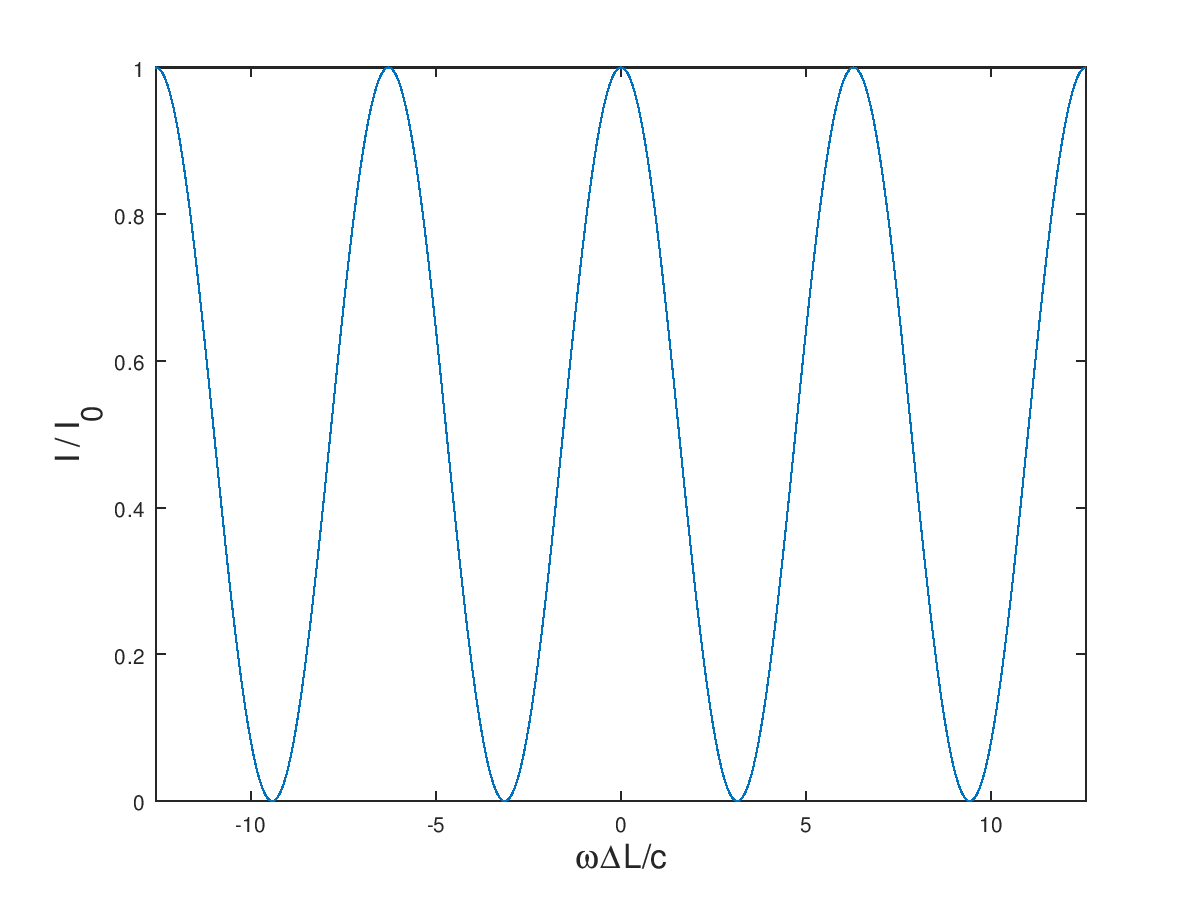
\includegraphics[width=.9\columnwidth]{OutputWithoutCell.png}
    \caption{无铷蒸汽腔的情况下,光电二极管输出随$\omega\Delta L/c$变化的关系(理论)}
        \label{OutputWithoutRbCell}
\end{figure}

当存在长度为$\Delta z$的铷蒸汽腔,折射率为$n=n_0(1+i\kappa)$的铷蒸汽会给B路光束在原有相位上带来额外的相位差(广义上的相位差,包含了衰减,为一复数):
\begin{align}
    e^{\frac{\omega}{c}(n-1)\Delta z}=e^{i\frac{\omega}{c}}e^{-\frac{\omega}{c}n_0\kappa\Delta z}=e^{i\delta}e^{-\tau},
\end{align}
其中铷蒸汽的吸收系数(传播单位距离光强衰减的百分比)
\begin{align}
    \notag\tau=&\frac{\omega}{c}n_0\kappa\Delta z=\frac{\omega}{c}\frac{\pi Nfe^2}{mV}\frac{\gamma/\omega_0}{\Delta\omega^2+\gamma^2}\\
    \approx&\frac{\pi Nfe^2}{cmV\gamma}\frac{\gamma^2}{\Delta\omega^2+\gamma^2}=\frac{\tau_0\gamma^2}{\Delta\omega^2+\gamma^2},
\end{align}
相移
\begin{align}
    \notag\delta=&\frac{\omega}{c}(n_0-1)\Delta z=-\frac{\omega}{c}\frac{\pi Nfe^2}{mV}\frac{\Delta\omega/\omega_0}{\Delta\omega^2+\gamma^2}\\
    \approx&-\frac{\pi Nfe^2}{cmV\gamma}\frac{\Delta\omega\gamma}{\Delta\omega^2+\gamma^2}=-\frac{\tau_0\Delta\omega\gamma}{\Delta\omega^2+\gamma^2},
\end{align}
以上约等号成立的条件为$\omega\approx\omega_0$,其中
\begin{align}
    \tau_0=\frac{\pi Nfe^2}{cmV\gamma}.
\end{align}
相移和吸收系数两者之间具有关系:
\begin{align}
    \delta=-\tau\frac{\Delta\omega}{\tau}.
\end{align}
此时A、B两路光束再次叠加时得到的电场分量为
\begin{align}
    E=\frac{E_0}{2}e^{i\frac{\omega}{c}L_1}+\frac{E_0}{2}e^{-\tau}e^{i\frac{\omega}{c}L_2}e^{i\delta}.
\end{align}
干涉光强与入射光强的比值为
\begin{align}
    \frac{I}{I_0}=\frac{\abs{E}^2}{E_0^2}=\frac{1}{4}\left[1+e^{-2\tau}+e^{-\tau}\cos\left(\frac{\omega}{c}\Delta L+\delta\right)\right].
\end{align}
对于$\tau_0$和$\Delta L$的不同取值,我们可以得到干涉光强随入射激光频率的各式变化关系,如图\ref{output-with-cell}所示. 若$\tau=0$,$\delta=0$,上式即为无铷蒸汽腔的情况推出的式\eqref{I/I_0-without-cell}.
\begin{figure}[H]
    \centering
    \subfigure[$\tau_0=0.4$]{
    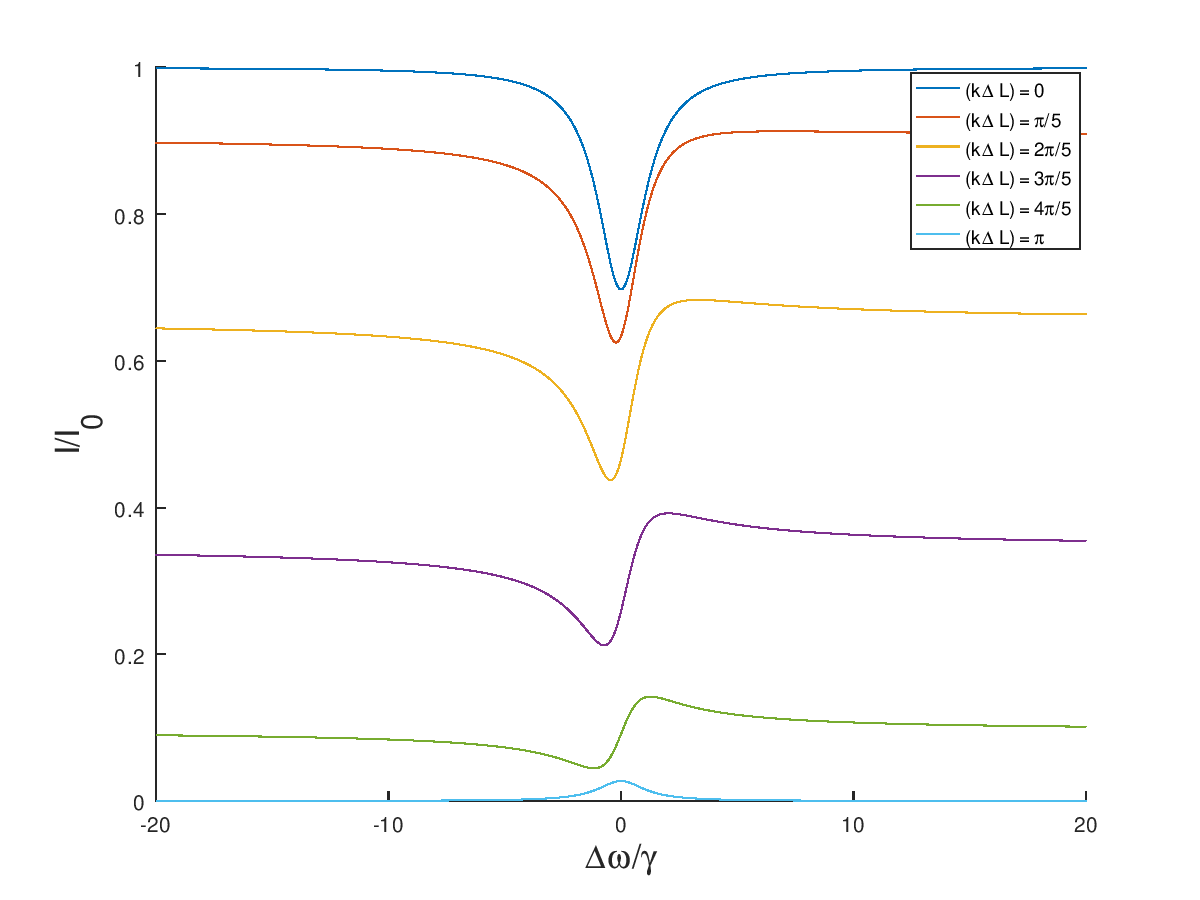
\includegraphics[width=0.9\columnwidth]{OutputWithCell-1.png}}
    \subfigure[$\tau_0=2$]{
    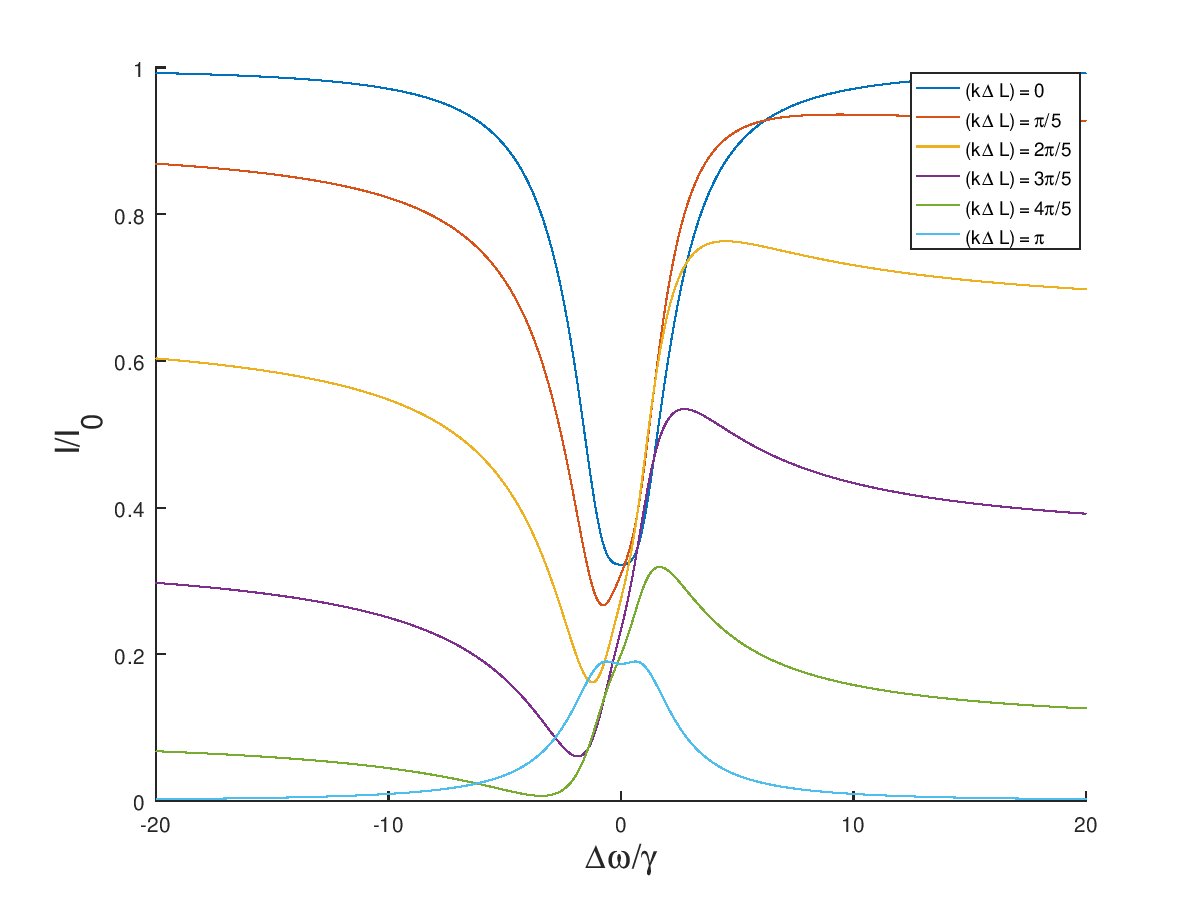
\includegraphics[width=0.9\columnwidth]{OutputWithCell-2.png}}
    \subfigure[$\tau_0=20$]{
    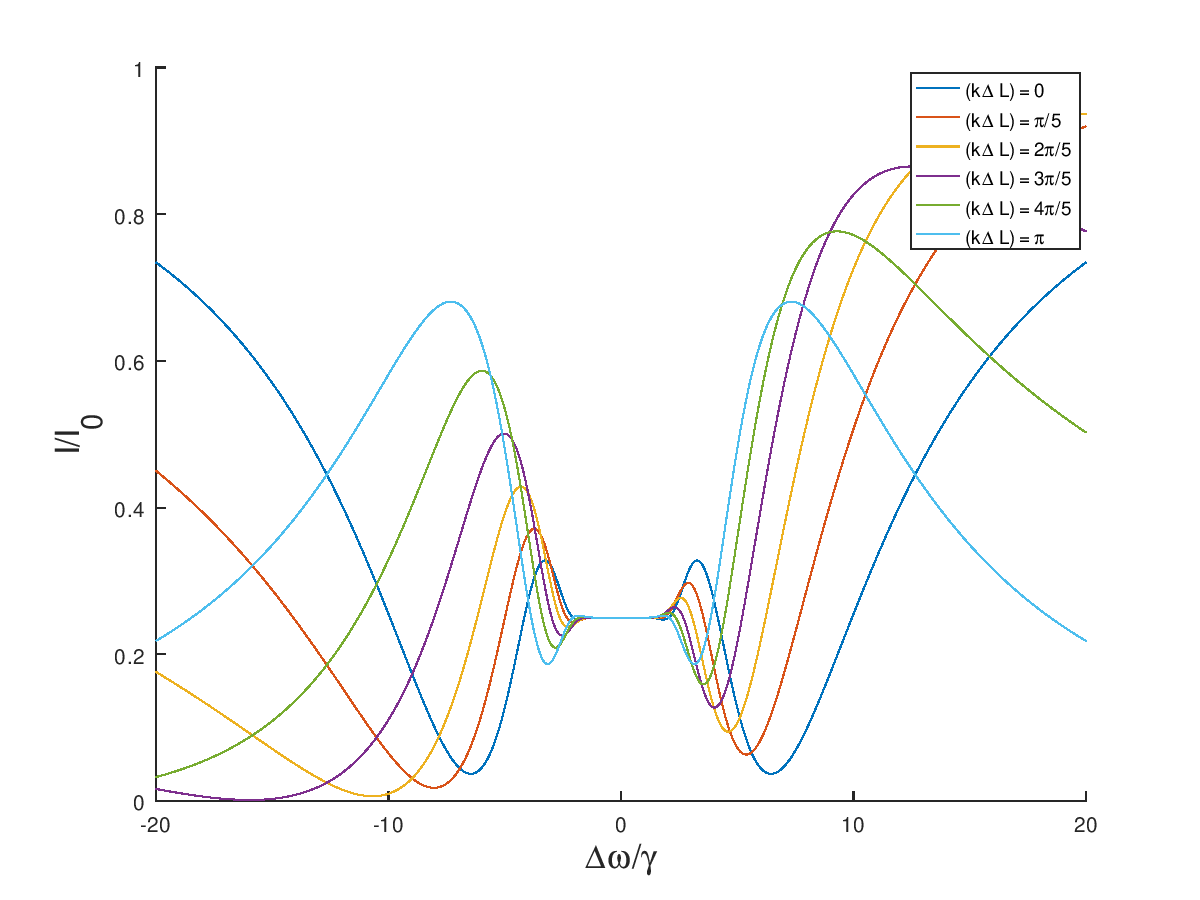
\includegraphics[width=0.9\columnwidth]{OutputWithCell-3.png}}
    \caption{干涉光强随入射激光频率的变化关系(理论)}
    \label{output-with-cell}
\end{figure}

理论上,Michelson干涉仪也可以完成与Mach-Zehnder干涉仪同样的测量任务,而且更方便调节单条光路的距离. 然而我们在预实验中发现,由于在Michelson干涉仪的每条光路中激光都沿着几乎重叠的路径往返各一次,很容易发生自发的饱和吸收,影响谱线的测量效果,因此总体看来还是Mach-Zehnder干涉更能胜任本实验的需求.

\section{实验测量与验证}

\subsection{利用饱和吸收法测量铷蒸汽吸收谱}

\subsubsection{实验设定}

\subsubsection{结果与分析}

\subsection{利用Mach-Zehnder干涉仪验证折射率的Kramers-Kronig关系}

\subsubsection{实验设定}

\subsubsection{结果与分析}

\section{结论}

\section{反思}

\begin{appendix}
\section{参考文献}
\nocite{*}
\bibliographystyle{plain}
\bibliography{References}
\end{appendix}
\end{multicols}
\end{document}